\documentclass[tikz]{standalone}

\usepackage{amsfonts}
\usepackage{amsmath}
\usepackage{braket}

\usepackage{tikz}
\usetikzlibrary{shapes.geometric,patterns,positioning,matrix}
\usetikzlibrary{shadows,calc,3d,arrows.meta,decorations.pathmorphing,decorations.markings,decorations.pathreplacing}

\definecolor{googleB}{HTML}{4285F4}
\definecolor{googleG}{HTML}{34A853}
\definecolor{googleY}{HTML}{FBBC05}
\definecolor{googleR}{HTML}{EA4335}
\definecolor{googleBG}{HTML}{3B96A4}

% load TikZ grafic definitions
%\input{gfx_TikZ}

% main document
\begin{document}

	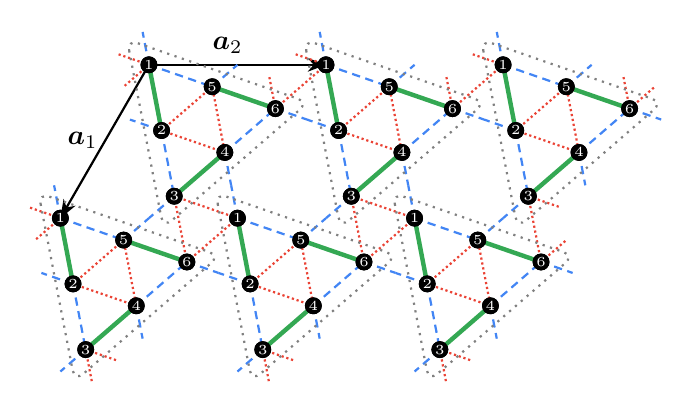
\begin{tikzpicture}

		\def\clipX{2.00}
		\def\clipY{1.75}
		\def\legLength{0.85}
		\def\tensorSize{0.1}
		\def\alpha{19.1066}

		% lattice vectors
		\begin{scope}[shift = {(0, 0)}]
            \draw[thick, -{Stealth[scale = 1.0]}] (0, 0) to ({-1*cos(30)*\legLength*sin(30)/sin(\alpha)}, {-2*cos(30)*tan(60)/2*\legLength*sin(30)/sin(\alpha)}) node at ($(240 : 1.25) + (150 : 0.25)$) {$\boldsymbol{a}_1$};
            \draw[thick, -{Stealth[scale = 1.0]}] (0, 0) to ({+2*cos(30)*\legLength*sin(30)/sin(\alpha)}, {+0*cos(30)*tan(60)/2*\legLength*sin(30)/sin(\alpha)}) node at ($(  0 : 1.00) + ( 90 : 0.25)$) {$\boldsymbol{a}_2$};
        \end{scope}

		% maple-leaf unit cells
		\begin{scope}[shift = {(0, 0)}]

			\foreach \x/\y in {0/0, 2/0, 4/0, -1/-2, +1/-2, +3/-2} {

				\begin{scope}[shift = {({\x*cos(30)*\legLength*sin(30)/sin(\alpha)}, {\y*cos(30)*tan(60)/2*\legLength*sin(30)/sin(\alpha)}, 0)}]

					\coordinate (1) at (0, 0);
					\coordinate (2) at ({-\alpha - 60} : {1*\legLength});
					\coordinate (3) at ({-\alpha - 60} : {2*\legLength});
					\coordinate (4) at ($(2) + ({-\alpha} : \legLength)$);
					\coordinate (5) at ($(1) + ({-\alpha} : \legLength)$);
					\coordinate (6) at ({-\alpha} : {2*\legLength});

					% internal links
					\draw[ultra thick, googleG] (1) to (2);
					\draw[ultra thick, googleG] (3) to (4);
					\draw[ultra thick, googleG] (5) to (6);
					\draw[thick, googleB, densely dashed] (1) to (5);
					\draw[thick, googleB, densely dashed] (2) to (3);
					\draw[thick, googleB, densely dashed] (4) to (6);
					\draw[thick, googleR, densely dotted] (2) to (5) to (4) to (2);

					% external links
					\draw[thick, googleB, densely dashed] (1) to ($(1) + ({120 - \alpha} : 0.5 * \legLength)$);
					\draw[thick, googleR, densely dotted] (1) to ($(1) + ({180 - \alpha} : 0.5 * \legLength)$);
					\draw[thick, googleR, densely dotted] (1) to ($(1) + ({240 - \alpha} : 0.5 * \legLength)$);

					\draw[thick, googleB, densely dashed] (2) to ($(2) + ({180 - \alpha} : 0.5 * \legLength)$);

					\draw[thick, googleB, densely dashed] (3) to ($(3) + ({240 - \alpha} : 0.5 * \legLength)$);
					\draw[thick, googleR, densely dotted] (3) to ($(3) + ({300 - \alpha} : 0.5 * \legLength)$);
					\draw[thick, googleR, densely dotted] (3) to ($(3) + ({360 - \alpha} : 0.5 * \legLength)$);

					\draw[thick, googleB, densely dashed] (4) to ($(4) + ({300 - \alpha} : 0.5 * \legLength)$);

					\draw[thick, googleB, densely dashed] (5) to ($(5) + ({ 60 - \alpha} : 0.5 * \legLength)$);

					\draw[thick, googleB, densely dashed] (6) to ($(6) + ({360 - \alpha} : 0.5 * \legLength)$);
					\draw[thick, googleR, densely dotted] (6) to ($(6) + ({ 60 - \alpha} : 0.5 * \legLength)$);
					\draw[thick, googleR, densely dotted] (6) to ($(6) + ({120 - \alpha} : 0.5 * \legLength)$);

					% lattice site
					\foreach \siteIdx in {1, 2, 3, 4, 5, 6} {
						\draw[black, fill = black] (\siteIdx) circle (\tensorSize);
						\draw[black, fill = black] (\siteIdx) circle (\tensorSize) node[white] at (\siteIdx) {\tiny$\siteIdx$};
					}

					\draw[thick, gray, dotted, rounded corners] ($(1) + ({150 - \alpha} : 0.5 * \legLength)$) to ($(3) + ({270 - \alpha} : 0.5 * \legLength)$) to ($(6) + ({ 30 - \alpha} : 0.5 * \legLength)$) -- cycle;

				\end{scope}

			}

		\end{scope}

	\end{tikzpicture}

\end{document}

%%% Local Variables:
%%% mode: latex
%%% TeX-master: t
%%% End:
